\chapter{Examples}

\section{$\pi$}

The code for this program is available in the appendix \ref{pi}.

\section{Enumeration sort}

The plot \ref{enumsort_plot} presents the speedup got parallelizing the differents loops.

\begin{figure}[!h]
  \begin{center}
         \resizebox{160mm}{!}{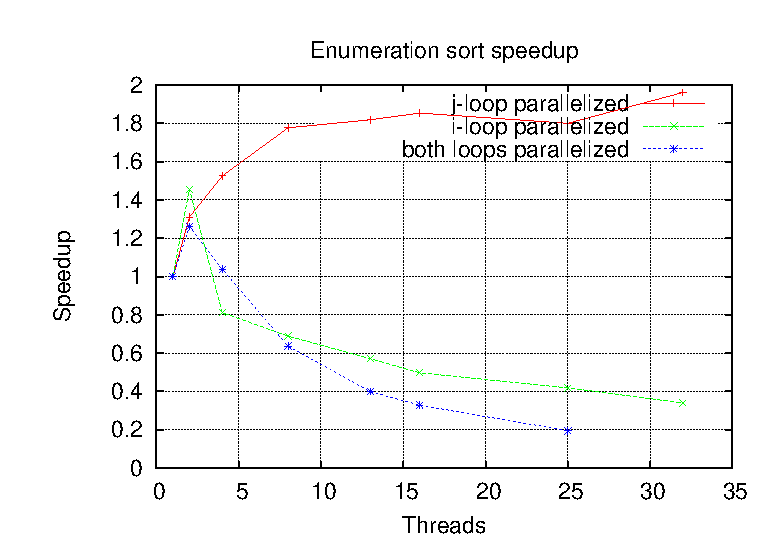
\includegraphics{pic/graph_enumsort.eps}}
  \end{center}
  \caption{enumeration sort's speedup}
  \label{enumsort_plot}
\end{figure} 

As we can see, the results are really bad when either the i-loop or both lopps are parallelized. In this case, the more threads we have, the more time we need to complete. We can also underline the fact that the program takes more time in that case than that it takes with only one thread. The only good result is given by parallelizing the $j$-loop only. This can be explained by the fact that the threads synchronize a lot among them in the two last cases.\\

When only the $j$-loop is parallelized, there is only one barrier at the end of the loop, that is one barrier in the whole program. So, the threads have to synchronize only once, hence the better performances.

However, in the case where the $i$-loop is parallelized, there is a barrier at the end of this loop. The problem comes from the fact that this loop is nested in the $j$-loop. So, there is a barrier for each $j$. Besides, there is a reduction operation. Thus, there is also some communication going on at that step. The time lost synchronizing the threads for each iteration and passing data around explains the bad results.

The very bad results at the last experiment are explained in the same way as above but this time both of the mentioned inconveniences are present. Because of the nested parallelization, not only the outer loop is divided among the threads but so is the inner loop. That means a barrier for each $j$ (plus a reduction) and a barrier at the end of the program. Therefore, there is again a lot of time wasted waiting for the others, hence the results.     
